\documentclass[journal,transmag]{IEEEtran}

% ..........................................................................
% Packages, configuration settings, and macro definitions.

\usepackage[pdftex]{graphicx}
\graphicspath{figures}
\DeclareGraphicsExtensions{.pdf,.jpeg,.png}

\usepackage[pdftex,rgb,dvipsnames,svgnames,hyperref,table]{xcolor}

\usepackage[pdftex,breaklinks=true,colorlinks=true,
	bookmarks=false,pdfhighlight=/O,
	urlcolor=DarkBlue,citecolor=DarkRed,linkcolor=DarkBlue]{hyperref}

\usepackage[cmex10]{amsmath}
\interdisplaylinepenalty=2500

\usepackage{amssymb}
\usepackage{amsfonts}
\usepackage{multicol}
\usepackage{multirow}
\usepackage{enumitem}
\usepackage{accsupp}
\usepackage{array}
\usepackage[caption=false,font=footnotesize]{subfig}
\usepackage{booktabs}
\usepackage{xspace}
\usepackage{soul}
\usepackage{url}
\usepackage{hyphenat}
\usepackage[english]{babel}

% Correct bad hyphenation here
\hyphenation{op-tical net-works semi-conduc-tor ana-ly-tics}

\usepackage{pdfcomment}
\newcommand{\comment}[3]{\pdfmarkupcomment[markup=Highlight,color=yellow,author={#2}]{#1}{#3}}

\usepackage{tabularx}
% ..........................................................................
% Body.

\begin{document}

\markboth{IEEE Transactions on Biomedical Engineering}{Standards for whole-cell modeling}

\title{Toward standards for tomorrow's whole-cell models}

\author{
	\IEEEauthorblockN{
		Dagmar Waltemath\IEEEauthorrefmark{1},
		Falk Schreiber\IEEEauthorrefmark{2,3}, 
		Jonathan R. Karr\IEEEauthorrefmark{4}, 
		Chris J. Myers\IEEEauthorrefmark{5},
%        Michael Hucka\IEEEauthorrefmark{6},       
%        Frank T. Bergmann\IEEEauthorrefmark{6,7,8},\\
        Vijayalakshmi Chelliah\IEEEauthorrefmark{9},\\
%        Marcus Krantz\IEEEauthorrefmark{10},
        Wolfram Liebermeister\IEEEauthorrefmark{11},
%        Pedro Mendes\IEEEauthorrefmark{12--15},
%        Pinar Pir\IEEEauthorrefmark{16},
        Begum Alaybeyoglu\IEEEauthorrefmark{17},
        Arne T. Bittig\IEEEauthorrefmark{18},
        Yin Hoon Chew\IEEEauthorrefmark{19},
        Rafael S. Costa\IEEEauthorrefmark{20},\\
        Muhammad Haseeb\IEEEauthorrefmark{21},
		Denis Kazakiewic\IEEEauthorrefmark{22,23},
		Ilya Kiselev\IEEEauthorrefmark{24},
        Vincent Knight-Schrijver\IEEEauthorrefmark{16},
		Christian Kn\"{u}pfer\IEEEauthorrefmark{25},\\
        Matthias K\"{o}nig\IEEEauthorrefmark{11},
		Nikita Mandrik\IEEEauthorrefmark{26},
        J. Kyle Medley\IEEEauthorrefmark{27},
        Sucheendra K. Palaniappan\IEEEauthorrefmark{28}, 
        Martin Scharm\IEEEauthorrefmark{1},\\
        Kieran Smallbone\IEEEauthorrefmark{29},
		Je-Hoon Song\IEEEauthorrefmark{30},
		Tom Theile\IEEEauthorrefmark{1},
        Namrata Tomar\IEEEauthorrefmark{31},
        Jannis Uhlendorf\IEEEauthorrefmark{10} and
        Markus Wolfien\IEEEauthorrefmark{1}
        }
	
	\IEEEauthorblockA{\IEEEauthorrefmark{1}Department of Systems Biology and Bioinformatics, University of Rostock}
	\IEEEauthorblockA{\IEEEauthorrefmark{2}Clayton School of Information Technology, Monash University}
    \IEEEauthorblockA{\IEEEauthorrefmark{3}Institute of Computer Science, Martin Luther University Halle-Wittenberg}    
	\IEEEauthorblockA{\IEEEauthorrefmark{4}Department of Genetics \& Genomic Sciences, Icahn School of Medicine at Mount Sinai} 
        %New York, NY 10029 USA\\Email: \href{mailto:karr@mssm.edu}{karr@mssm.edu}
    \IEEEauthorblockA{\IEEEauthorrefmark{6}Department of Electrical and Computer Engineering, University of Utah} 
        %Salt Lake City, Utah 84112, USA
%    \IEEEauthorblockA{\IEEEauthorrefmark{5}Department of Computing and Mathematical Sciences, California Institute of Technology} 
        %1200 East California Boulevard, Pasadena, CA 91125, USA
%    \IEEEauthorblockA{\IEEEauthorrefmark{7}BioQuant, University of Heidelberg} 
        %Heidelberg , Germany
%    \IEEEauthorblockA{\IEEEauthorrefmark{8}Centre for Organismal Studies, University of Heidelberg} 
    \IEEEauthorblockA{\IEEEauthorrefmark{9}European Molecular Biology Laboratory, European Bioinformatics Institute} 
        %Wellcome Trust Genome Campus, Hinxton, Cambridge CB10 1SD, UK viji@ebi.ac.uk.
    \IEEEauthorblockA{\IEEEauthorrefmark{10}Department of Biology, Humboldt University of Berlin} 
        %Berlin, Germany
    \IEEEauthorblockA{\IEEEauthorrefmark{11}Institute of Biochemistry, University Medicine Charit\'{e} Berlin, 10117 Berlin, Germany}
        %10117 Berlin, Germany
%    \IEEEauthorblockA{\IEEEauthorrefmark{12}Manchester Institute of Biotechnology, University of Manchester} 
%    \IEEEauthorblockA{\IEEEauthorrefmark{13}School of Computer Science, University of Manchester}     
%    \IEEEauthorblockA{\IEEEauthorrefmark{14}Center for Quantitative Medicine, University of Connecticut Health Center}
%    \IEEEauthorblockA{\IEEEauthorrefmark{15}Department of Cell Biology, University of Connecticut Health Center}
        %131 Princess Street, Manchester, M1 7DN, UK. pedro.mendes@manchester.ac.uk
        %Farmington, Connecticut, USA
    \IEEEauthorblockA{\IEEEauthorrefmark{16}Babraham Institute}
    \IEEEauthorblockA{\IEEEauthorrefmark{17}Department of Chemical Engineering, Bo\v{g}azi\c{c}i University}
	\IEEEauthorblockA{\IEEEauthorrefmark{18}Modeling and Simulation Group, Institute of Computer Science, University of Rostock}	
    \IEEEauthorblockA{\IEEEauthorrefmark{19}Centre for Synthetic and Systems Biology, University of Edinburgh}
    \IEEEauthorblockA{\IEEEauthorrefmark{20}Instituto Superior T\'ecnico, University of Lisbon}
    \IEEEauthorblockA{\IEEEauthorrefmark{21}Department of Bioinformatics, Mohammad Ali Jinnah University}
	\IEEEauthorblockA{\IEEEauthorrefmark{22}Center for Statistics, Universiteit Hasselt, Hasselt BE3500, Belgium}
    \IEEEauthorblockA{\IEEEauthorrefmark{23}Center for Innovative Research, Medical University of Bialystok, Bialystok 15-089, Poland}
	\IEEEauthorblockA{\IEEEauthorrefmark{24}Design Technological Institute of Digital Techniques of the Siberian Branch of the Russian Academy of Sciences, Novosibirsk}
	\IEEEauthorblockA{\IEEEauthorrefmark{25}Institut f\"ur Informatik, University of Jena}
	\IEEEauthorblockA{\IEEEauthorrefmark{26}Sobolev Institute of Mathematics, Siberian Branch of the Russian Academy of Sciences, Novosibirsk}	
	\IEEEauthorblockA{\IEEEauthorrefmark{27}Department of Bioengineering, University of Washington, Seattle, WA 98195, USA}	
    \IEEEauthorblockA{\IEEEauthorrefmark{28}Rennes - Bretagne Atlantique Research Centre, Institute for Research in Computer Science and Automation}	
    \IEEEauthorblockA{\IEEEauthorrefmark{29}Manchester Centre for Integrative Systems Biology, University of Manchester}    	
	\IEEEauthorblockA{\IEEEauthorrefmark{30}Department of Bio and Brain Engineering, Korea Advanced Institute of Science and Technology}
	% (KAIST),\\ 291 Daehak-ro, Yuseong-gu, Daejeon 305-701, Republic of Korea	
    \IEEEauthorblockA{\IEEEauthorrefmark{31}Department of Dermatology, University Medicine, University of Erlangen-Nuremberg}
    %\\ Hartmannstraße 14, 91052 Erlangen, Germany
    
	\thanks{Corresponding author email: \href{mailto:dagmar.waltemath@uni-rostock.de}{dagmar.waltemath@uni-rostock.de}}
}

\IEEEtitleabstractindextext{
	\begin{abstract}
	Whole-cell models are promising tools for biological research, bioengineering, and medicine. 
	However, significant work remains to achieve complete and accurate whole-cell models, including developing a strong theoretical understanding of multi-algorithm modeling, a standardized whole-cell modeling language, and an efficient general-purpose simulator.
	We organized the 2015 Whole-Cell Modeling Summer School to teach whole-cell modeling, as well as to evaluate the need for new whole-cell modeling standards by attempting to encode a recently published whole-cell model into SBML.
    We propose three SBML extensions to support transparent, reproducible whole-cell modeling: support for multi-algorithm models, support for particle-based state representation, and support for template reactions. In addition, we describe several new software tools which are needed to enable researchers to encode and simulate whole-cell models including a user-friendly graphical model editor and a parallelized simulator. We also propose several new SGBN extensions.
	Together these new standards and software tools would accelerate whole-cell modeling.
	\end{abstract}
	
	\begin{IEEEkeywords}
	Whole-cell modeling, Systems biology, Computational biology, Mathematical modeling, Simulation, Standards, Education
	\end{IEEEkeywords}
}

\maketitle
\IEEEdisplaynontitleabstractindextext
\IEEEpeerreviewmaketitle

\section{Introduction}

\IEEEPARstart{O}{ver} the past twenty years, computational modeling has become an essential and powerful tool for biological research, bioengineering, and medicine to analyze high-throughput molecular measurements and understand the molecular details of complex biological systems. Computational modeling has  been used to identify new metabolic genes~\cite{Reed2006}, to add metabolic pathways to bacteria~\cite{Lee2012}, to and identify potential new antimicrobial drug targets~\cite{Lee2009}.
Computational models also have the potential to enable bioengineers to design new microorganisms for industrial applications such as chemical synthesis, biofuel production, and waste decontamination, as well as to enable clinicians to tailor therapy to individual patients. Realizing this potential requires more comprehensive and accurate computational models which are capable of predicting cellular behavior from genotype, as well as standardized methods for exchanging models, simulation experiments, and model visualizations~\cite{Macklin2014,Karr2015,hucka2015promoting,Klipp07}.

Recently, researchers at Stanford University developed the first whole-cell model of the gram-positive bacterium \textit{Mycoplasma genitalium}~\cite{Karr2012}. The model represents the life cycle of a single Mycoplasma cell including the copy number dynamics of each metabolite, RNA, and protein species and accounts for every known gene function. The model is composed of 28 sub-models, each of which is implemented using different mathematical representations including ordinary differential equations (\emph{ODE}s), flux balance analysis (\emph{FBA}), and Boolean rules (\emph{BR}s), and trained using different experimental data.

The \textit{M. genitalium} whole-cell model was implemented in MATLAB, is available open-source under the MIT license, and is extensively documented \cite{wholeCell}. This has enabled other researchers to use the model for their own research. 

However, the \textit{M. genitalium} whole-cell model software is not transparent or reusable. The \textit{M. genitalium} whole-cell model software is also not user-friendly, computationally efficient, or easily maintainable. Consequently, significant domain expertise is required to use the \textit{M. genitalium} model or construct new whole-cell models. New whole-cell modeling standards and simulation tools are needed to enable more researchers to develop and simulate their own whole-cell models. Such standards and software tools would accelerate whole-cell modeling. They would enable researchers to develop models more quickly, to explore models more deeply, and to evaluate models more rigorously. Furthermore, standards would simplify the submission process to model repositories such as BioModels~\cite{juty2015biomodels,chelliah2015biomodels}. In turn, this would make models more searchable, retrievable, reusable, and comparable.

Several systems biology standards have already been developed by the COmputational Modeling in BIology NEtwork (\emph{COMBINE})~\cite{le2011meeting} including the Systems Biology Markup Language (\emph{SBML})~\cite{hucka2003}, the Cell Markup Language (\emph{CellML})~\cite{hedley_2001b}, the Simulation Experiment Description Markup Language (\emph{SED-ML})~\cite{sedml2011}, and the Systems Biology Graphical Notation (\emph{SBGN})~\cite{LeNovereHMMSS09}. SBML and CellML are languages for describing mathematical models including ODE, logical, and FBA models. Both have been used to build thousands of models of various intracellular pathways. SED-ML is a language for describing computational experiments. SED-ML enables scientists to reproduce a simulations by completely describing simulation setups, including the simulation algorithm and every parameter value. SBGN includes three languages for describing visual representations of models. None of these standards have been used to construct, simulate, or visualize models as complex as the \textit{M. genitalium} whole-cell model.

We organized the 2015 Whole-Cell Modeling Summer School to train students in whole-cell modeling, as well as to evaluate the need for new standards for whole-cell modeling. The majority of the school was focused on trying to encode the \textit{M. genitalium} whole-cell model using SBML to train students, as well as to evaluate the ability of SBML to encode whole-cell models. The ultimate scientific goal of the school was to develop an open-source whole-cell model encoded in SBML and simulated using SED-ML.

Here, we describe the summer school, outline our progress toward encoding the \textit{M. genitalium} model using SBML, and propose several SBML and SGBN extensions to support whole-cell modeling. First, we summarize the summer school. Second, we describe our progress toward encoding the \textit{M. genitalium} whole-cell model using SBML. Lastly, we describe the SBML and SBGN expansions and software tools needed to support whole-cell modeling.

\section{The 2015 Whole-Cell Modeling Summer School}
We organized the summer school to teach students how to build and encode models using COMBINE standards by attempting to encode the \textit{M. genitalium} model using only standard representation formats.

\subsection{Organization}
The Whole-Cell Modeling Summer School was held March 9-13, 2015 at the University of Rostock in Rostock, Germany. The school was organized by Dagmar Waltemath and Falk Schreiber and supported by the Volkswagen Foundation. 45 students, nine instructors, and two organizers participated in the five-day school.

The school began with two lectures which introduced whole-cell modeling and the existing systems biology standards. Jonathan Karr from the Icahn School of Medicine at Mount Sinai, USA presented an overview of whole-cell and multi-algorithm modeling. Michael Hucka from the California Institute of Technology, USA presented an overview of the SBML, SED-ML, and SBGN standards; several open-source software tools which support these standards; and the COMBINE initiative. We also organized three discussions on multi-algorithm model composition, particle-based state representation, and random number generation. 

The majority of the school was dedicated to hands-on active learning sessions in which students learned about whole-cell modeling and the COMBINE standards by trying to encode parts of the \textit{M. genitalium} whole-cell model using SBML. Students were divided into ten groups of four to five students, each of which was challenged to encode one or more sub-models using SBML. Each group was led by an experienced instructor.

Each day concluded with brief progress reports from each group. This facilitated discussion on common encoding challenges and model integration and provided an opportunity for groups to obtain feedback from each other.

We also organized a poster session, as well as several evening social activities to provide the students opportunities to network with each other and the instructors.

\subsection{Educational outcomes}
\comment{We surveyed the students to assess the educational outcome of the school.}{Karr}{What did the survey actually show?}
Most students reported gaining deep knowledge of whole-cell modeling, increased appreciation for reproducible science, and increased understanding of the SBML, SED-ML, and SBGN standards. Many students also reported learning about open-source modeling software tools relevant to their own research.

In addition, many of the students reported that the school expanded their scientific network. Several students commented that the school introduced them to potential postdoctoral positions and next year's whole-cell modeling summer school (\href{http://www.wholecell.org/school-2016}{http://www.wholecell.org/school-2016}).

\subsection{Lessons learned for organizing research-based schools}
We learned several valuable lessons about how to best organize an open-ended, research-based school. First, we conclude that research-based schools should clearly outline the expected background knowledge and learning objectives and have well-organized learning activities. This helps students make informed decisions about whether to participate in the school, know how to prepare for the school, and learn efficiently.
Second, we conclude that students greatly enjoy learning through open research problems rather than through prescribed training exercises. This makes students feel engaged, challenged, and connected to research. This also helps students build practical skills to complement their foundational undergraduate and graduate training.
Third, we conclude that open-ended project-based schools require a high teacher-to-student ratio, a flexible schedule, and multidisciplinary project teams. A high teacher to student ratio allows students to get feedback and iterate through potential solutions quickly. A flexible schedule enables impromptu lectures and discussions. Multidisciplinary teams enable students to work through difficult problems by drawing on perspectives from multiple fields. 

\section{Toward an SBML-encoded whole-cell model}
In addition to training young computational systems biology researchers, the second goal of the school was to attempt to encode the \textit{M. genitalium} whole-cell model (\url{https://github.com/CovertLab/WholeCell/releases/tag/v1.1}) into SBML. To achieve this goal, most of the course was devoted to active learning sessions in which students were challenged to encode sub-models of the \textit{M. genitalium} into SBML, integrate sub-models into a single model, and simulate models using SED-ML. During these sessions, the students and instructors were divided into ten groups. Eight of the groups were tasked with encoding one or more sub-models. The ninth group was tasked with developing a standards-compliant scheme to integrate the sub-models into a single model. This group was responsible for defining the global state variables and sub-model interfaces and developing a SED-ML scheme to simulate the integrated model. The tenth group was responsible for developing an annotation scheme and helping the other groups document and visualize their sub-models. Table~SI lists the ten groups and all of the students and instructors. 

\subsection{Sub-model encoding}
The eight sub-model encoding groups pursued various strategies to encode the sub-models using SBML. Several of the groups encoded sub-models by first reading the sub-model documentation, then drawing pathway maps using software tools such as Cell Designer~\cite{funahashi2008celldesigner} and VANTED~\cite{Rohn2012}, and finally writing scripts to generate SBML models from their maps. Other groups used modeling software tools such as BioUML~\cite{Kolpakov2006}, COPASI~\cite{Mendes2009}, and iBioSim~\cite{Madsen2012} to encode sub-models based on their documentation. A few of the groups encoded sub-models by converting the MATLAB code to SBML. These groups then generated SBGN maps from their SBML to better understand their sub-models.

The groups encountered several challenges to encoding the \textit{M. genitalium} sub-models into SBML. First, most of the groups had to spend a significant amount of time reading the MATLAB code and documentation to understand the details of the \textit{M. genitalium} sub-models because the connection between the sub-models and the associated pathway/genome database is not transparent, many of the sub-models details are implemented directly in MATLAB code rather than in a transparent language such as SBML, and the documentation only provides overviews of the sub-models. Fortunately, one of the authors of the \textit{M. genitalium} model was available to answer questions about the model.

A second challenge to encoding the sub-models in SBML was encoding serially executed MATLAB sub-models into SBML which, because it is not a programming language, does not expose control over the order of simulation execution. This fundamental difference between programming languages and SBML makes quantitatively reproducing the \textit{M. genitalium} model impossible. Most of the groups decided to tackle this problem by formalizing MATLAB sub-models as discrete stochastic models and simulating them using the Gillespie or other approximate algorithms. For several of the sub-models, this conversion imposed an explicit internal sub-model timescale which was not present in the original MATLAB sub-model due to the lack of kinetic data for the corresponding pathway.

The fact that SBML is not a programming language and does not expose methods for arbitrary random number generation also made it challenging for groups to encode the random algorithms used by the MATLAB sub-models into SBML. For example, the MATLAB translation sub-model includes a random algorithm which assigns amino acids to individual polypeptides. Because this algorithm is not equivalent to othe Gillespie algorithm, the algorithm cannot easily be encoded into SBML. Most of the groups also solved this problem by formalizing sub-models as stochastic models. Even if it were possible to transcode the MATLAB sub-models directly into SBML, it would still be difficult to quantitatively reproduce the MATLAB simulations because SBML does not expose control over the random number generator algorithm or seed. Consequently, it would only be feasible to compare the first two moments of the MATLAB and transcoded model simulations.

To encode many of the sub-models into SBML, the groups also had to either enumerate the hybrid population/particle-based state representation used by the MATLAB sub-models or approximate the MATLAB sub-models. The groups responsible for the transcription and translation sub-models chose to approximate the MATLAB sub-models by eliminating the internal dynamics of the polymerization of each RNA and polypeptide. Consequently, these sub-models no longer track the progress of individual RNA polymerases and ribosomes, account for base-specific transcription or translation rates, or predict RNA polymerase collisions. The groups responsible for the DNA sub-models including replication, replication initiation, and transcriptional regulation, chose to enumerate the sparse chromosome representation used by the MATLAB model by creating Boolean indicator variables to represent the existence and protein-binding status of each chromosome base. This enumerated representation requires millions of variables. Consequently, the corresponding SBML XML files are impractical to read and computationally expensive to simulate. Enumerating the rules which govern the joint values of the enumerated variables, such as the rules which represent the steric effects of DNA-bound proteins by preventing proteins from binding neighboring bases, is also impractical. Furthermore, the enumerated SBML files are impractical for humans to read, edit, or maintain.

The lack of universal SBML simulator support for arrays was another challenge to encoding the MATLAB sub-models into SBML. All of the groups overcame the lack of array support by enumerating individual array elements of the MATLAB and all matrix algebra computations. This creates verbose SBML files which are more difficult to interpret, maintain, and edit. Enumerating the matrix algebra computations also increases the computational cost of simulation.

Together, these five challenges made it very difficult for the groups to encode most of the MATLAB sub-models into SBML. Going forward, SBML and the SBML simulators should be expanded to provide support for random number generation, particle-based state representation, and arrays.

\subsection{Model integration}
The integration group was responsible for assembling the individual sub-models into a single model including defining the global state variables, defining the interfaces exposed by the sub-models to the global state variables, and developing a scheme for managing simultaneous writing of shared state variables. The integration group defined the global state variables as the union of all state variables shared by at least two sub-models rather than by explicitly defining a set of global state variables as done by the MATLAB simulator. The advantages of this approach are that sub-model developers are not also required to develop global state variables and that it minimizes the number of global state variables. The disadvantages of this approach are that the total set of variables is less transparent and that it requires users to learn all of the sub-models and their naming conventions to analyze model simulations.

The integration group standardized the interfaces exposed by the individual sub-models by defining a variable naming convention. This naming convention ensures, for example, that the copy numbers of each protein species are represented by variables with the same names in each of the sub-models. This convention makes it clear how multiple local sub-model variables map onto the same global variable. Specifically, the integration group chose to use the same variable names as those used by the MATLAB implementation. Matrix and particle-based variables were enumerated by creating multiple variables with names containing additional suffixes to indicate their identity.

The primary challenge faced by the integration group was how to handle concurrent editing of shared state variables by multiple sub-models. \comment{The integration group explored several potential strategies to manage concurrent writing.}{Karr}{Chris Myers, can you elaborate?} First, they explored sequentially simulating the sub-models and updating the global state variables. This avoids the need for more complex strategies to merge variable changes. However, under this approach sub-models are simulated with different variable values within each timestep. Consequently, simulation predictions are sensitive to the sub-model execution order. 

The integration group also explored several more complex sub-model integration strategies which enable all of the sub-models to be simulated with the same variable values within each timestep. These strategies included reducing the sub-model integration timestep such that sub-models do not request conflicting variable changes; dividing each of the shared state variables into separate, independent sub-variables for each sub-model, simulating the sub-models in parallel, and merging the sub-variables to compute the update global values; and using semaphores to manage concurrent variable changes whereby at each timestep sub-models request sets of atomic state variables changes and a controller decides which change sets are processed. Each of these strategies has different advantages and disadvantages. The first strategy is the simplest to understand and implement, but is computationally expensive. The second strategy is simple to implement and computationally efficient for independent variables, but is difficult to implement for sets of non-independent variables such as those which represent the protein occupancy of the chromosome. The third strategy is the most complex to implement, but is more general than the second strategy and more computationally efficient than the first. The integration group tested their sub-model integration strategies using iBioSim because iBioSim is one of the only SBML simulators to support all of the existing needed SBML packages including hierarchical model composition (\emph{comp}), arrays, and flux balance constraints (\emph{fbc}).

The lack of an SBML simulator which supports multi-algorithm model composition was another challenge to integrating the sub-models. The integration group plans to overcome this limitation by adding support for multi-algorithm to iBioSim.

\subsection{Progress}
The students produced preliminary SBML and SBGN-ML versions of many of the \textit{M. genitalium} whole-cell model sub-models. However, significant work remains to finish encoding the sub-models, integrate the sub-models into a single model, and test the sub-models and the combined model. Complete drafts are only available for a few of the simplest sub-models. The current drafts of most of the more complex sub-models are also greatly simplified compared to their MATLAB versions. For example, the transcription and translation sub-models drafts do not represent the polymerization of individual bases and the DNA sub-models do not account for the protein occupancy of the chromosome. In addition, none of the SBML-encoded sub-models have been thoroughly tested by replicating the unit tests from the MATLAB implementation. Furthermore, none of the SBML sub-models have been thoroughly documented and complete SBGN maps are not yet available for any of the sub-models.

\subsection{Future steps}
We hope to finish encoding the \textit{M. genitalium} sub-models into SBML and integrate the SBML-encoded sub-models into a single model simulatable by open-source software tools such as COPASI, BioUML, and iBioSim. Several students and instructors have continued to keep working and meeting online. Several students and instructors also plan to participate in a second meeting in October 2015 which will be held at the University of Utah, USA immediately prior to the 2015 COMBINE Forum.

Going forward, we plan to publish SBML-encoded versions of each of the \textit{M. genitalium} sub-models to BioModels, along with SED-ML tests, SBGN maps, and textual documentations. This would make the sub-models searchable, retrievable, and reusable by other scientists. We believe this would be a valuable community resource. It would demonstrate how to build a whole-cell model and enable other researchers to build upon the \textit{M. genitalium} sub-models. Ultimately, SBML and the SBML simulation software tools also need to be extended to facilitate whole-cell modeling.


\section{Toward SBML-, SED-ML-, and SBGN-based standards for whole-cell modeling}
Prior to the school, SBML, SED-ML, and SBGN had never been used to represent whole-cell or similarly complex models. Consequently, not surprisingly, the summer school revealed several limitations of SBML, SBGN, and the existing simulation software for large models. Importantly, the summer school facilitated discussions among modelers, tool developers, and model curators about how to best expand the existing standards and software tools to overcome these limitations.

\subsection{Current limitations}
As discussed above, SBML does not support multi-algorithm modeling, particle-based state representation, or arbitrary random number generation and the current SBML simulators have limited support for arrays. Consequently, SBML cannot efficiently simulate models with large, combinatorial state spaces; represent arbitrary stochastic models; or efficiently simulate arbitrary mathematical models involving matrix algebra operations. State spaces must be enumerated, stochastic models must be described using a ratio time scale and simulated using the Gillespie or other approximate algorithm, and matrix algebra operations must be expanded. For the \textit{M. genitalium} whole-cell model this would result in large, unmanageable XML files and millions of variables.

Furthermore, no general-purpose SBML simulation software is currently capable of efficiently simulating models involving millions of variables and no SBML simulation software supports multi-algorithm modeling. In addition, no SBML editing tool provides researchers a user-friendly interface for editing SBML files containing millions of variables. Consequently, currently, whole-cell model SBML files must be generated by scripts and cannot be easily edited.

The summer school also revealed several limitations of the graphical representation scheme SBGN and the existing SBGN viewers for whole-cell models. First, whole-cell modeling requires hybrid SBGN maps which contain all three types of nodes: Process Descriptions, Entity Relationships, and Activity Flows. Currently, SBGN maps can only contain one type of node. Second, whole-cell modeling requires new automatic layout algorithms suitable for large maps. The existing layout algorithms are unable to construct intuitive maps of many of the pathways that need to be in whole-cell models. Third, in order to effectively visualize complex SGBN maps of whole-cell models, SBGN viewers must be able to display maps at different levels of granularity by automatically reducing maps.

The summer school did not reveal any limitations of SED-ML for describing whole-cell model simulations.

\subsection{Standard extensions}
Taken together, expanded standards and supporting software tools are needed to facilitate accurate, reproducible whole-cell modeling. We propose three SBML expansions to facilitate whole-cell modeling. First, the SBML comp package must be expanded to support models composed of sub-models implemented with different simulation algorithms. Currently, the comp package only supports models composed of sub-models each implemented using the same simulation algorithm. In addition, the existing SBML simulators must be expanded to support multi-algorithm simulations and/or new simulators must be developed which support the expanded package. This requires significantly more research to determine the best ways to integrate heterogeneous sub-models, including rigorously evaluating the advantages and disadvantages of each of the schemes proposed by the integration group. Significant effort will also be needed to develop a parallelized simulator which is capable of quickly simulating complex whole-cell models.

Second, a new SBML package must be created to support hybrid population/particle-based state representations such as those used by BioNetGen \cite{Hlavacek2006, Hogg2014} and NFSim \cite{Sneddon2011}. In parallel, the existing SBML simulators must be expanded to support this new package and/or new SBML simulators must be developed. This would enable modelers to compactly describe and efficiently simulate models with large, combinatorial state spaces. The compact descriptions enabled by this package would also make models more transparent and easier to maintain and expand. 

A new SBML package must also be created to support reaction templates so that, for example, translation could be described using a single reaction template and arrays of mRNA-specific translation initiation rates and codon-specific elongation rates. Such reaction templates would enable whole-cell and other large models to be compactly described, and consequently easily interpretable, maintainable, and editable. By separating the mathematical descriptions and quantitative parameter values, reaction templates would also make the connection between dynamical models and the experimental data used to inform their parameter values more transparent. The new reaction templates could be expanded for backward compatibility with older SBML simulators.

New user-friendly graphical editors must also be developed to enable researchers to easily build SBML files which take advantage of these new features. These graphics editors must also allow researchers to transparently map model parameters onto experimental data organized in pathway/genome databases.

In addition, as discussed above, SBGN must be expanded to support hybrid diagrams and the SBGN viewers must be expanded to support more automatic layout algorithms, automatic model reduction, and contextual zooming. These features would enable researchers to use SBGN to map whole-cell and other large models.

Together, these SBML, SBGN, and software expansions would enable more researchers to more easily build, manage, simulate, and reproduce whole-cell models and simulations. These new standards and software tools would also enable researchers to build more comprehensive and more accurate models, including of human cells. Ultimately, these new standards and software would enable whole-cell modeling to support rational biological design and personalized medicine.

\section{Conclusion}
The 2016 Whole-Cell Modeling Summer School provided 45 young scientists hands-on training in whole-cell and multi-algorithm modeling through attempting to encode the \textit{M. genitalium} whole-cell model into SBML. Additional summer schools and courses are needed to provide students with deeper theoretical training in dynamical modeling, multi-algorithm modeling, model reduction, and parameter estimation, as well as practical training in model construction including data curation, model building, numerical optimization, model testing, and model analysis.

The summer school also made significant strides toward encoding the \textit{M. genitalium} whole-cell model using SBML for simulation by open-source software. The students developed preliminary SBML versions of all of the sub-models of the \textit{M. genitalium} model. Since the summer school, several students have continued to encode the \textit{M. genitalium} model, and several of the students and instructors are participating in a second meeting prior to 2015 COMBINE Forum at the University of Utah in Salt Lake City, USA. Ultimately, we hope to publish an SBML-encoded version of the model to BioModels. 

However, significant work remains to complete, test, integrate, simulate, and document the SBML-encoded version of the \textit{M. genitalium} model. Currently, SBML cannot represent whole-cell models, there is no simulation software program which could efficiently simulate an SBML-encoded whole-cell model, and there is no graphical editor which is capable of constructing, editing, or visualizing an SBML-encoded whole-cell model. SBML must be expanded to support multi-algorithm modeling, template reactions, particle-based state representation, and arrays and an efficient simulation software program and a user-friendly model editor must be developed to enable modelers to easily construct and simulate whole-cell models. New parameter estimation, model testing, and visual analysis tools must also be developed to enable researchers to effectively use SBML-encoded whole-cell models for scientific research. SBGN and the SBGN viewers must also be expanded to support hybrid diagrams, automatic graph layout, automatic graph reduction, and contextual zooming.

In summary, we believe that whole-cell modeling has the potential to be an important tool for biological discovery, bioengineering, and medicine. Achieving this potential requires improved standards for describing whole-cell models, as well as new general-purpose simulation software for reproducibly simulating whole-cell models. In turn, this requires expanding the whole-cell modeling field including training additional young researchers.

\section*{Acknowledgments}
The school was supported by a grant from the Volkswagen Foundation to DW and FS. JRK was supported by a James S. McDonnell Foundation Postdoctoral Fellowship Award in Studying Complex Systems.

\ifCLASSOPTIONcaptionsoff
  \newpage
\fi

\bibliographystyle{IEEEtran}
\bibliography{IEEEabrv,report}

% biography section
% 
% If you have an EPS/PDF photo (graphicx package needed) extra braces are needed around the contents of the optional argument to biography to prevent
% the LaTeX parser from getting confused when it sees the complicated \includegraphics command within an optional argument. (You could create
% your own custom macro containing the \includegraphics command to make things simpler here.)

\vskip0.25in
\begin{IEEEbiography}[{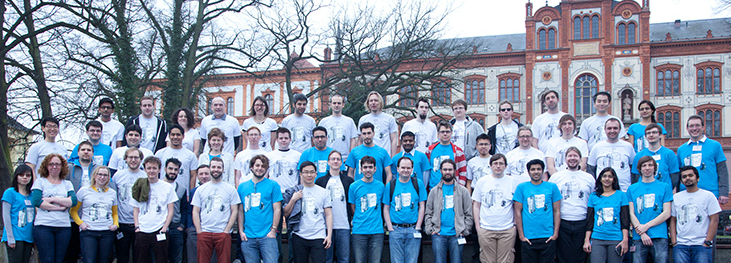
\includegraphics[width=516pt,keepaspectratio]{photos/group.jpg}}]{}
~\\
~\\
~\\
~\\
~\\
~\\
~\\
~\\
~\\
~\\
~\\
~\\
~\\
~\\
~\\
~\\
\textbf{2015 Whole-Cell Modeling Summer School} included the 56 researchers listed in Table~SI.
\end{IEEEbiography}


% You can push biographies down or up by placing a \vfill before or after them. The appropriate
% use of \vfill depends on what kind of text is on the last page and whether or not the columns are being equalized.

\vfill

% Can be used to pull up biographies so that the bottom of the last one is flush with the other column.
%\enlargethispage{-5in}

% ..........................................................................
% End.

\clearpage
\setcounter{table}{0}
\renewcommand{\thetable}{S\Roman{table}}

\begin{table*}[ht!]
\caption{2015 Whole-Cell Modeling Summer School participants.}
\begin{tabularx}{\textwidth}{l||l||X}\hline
\bfseries Group           & \bfseries Participant            & \bfseries Affiliation\\\hline\hline
Cytokinesis               & Naveen Kumar Aranganathan        & University Paris-Sud, France\\
                          & Daniel Alejandro Priego Espinosa & National Autonomous University of Mexico, Mexico\\
                          & Ilya Kiselev                     & Siberian Branch of the Russian Academy of Sciences Novosibirsk, Russia\\
                          & Wolfram Liebermeister            & Charit\'e Medical University of Berlin, Germany\\
                          & Yan Zhu                          & Monash University, Australia\\\hline
DNA repair                & Arne Bittig                      & University of Rostock, Germany\\
                          & Vijayalakshmi Chelliah           & European Bioinformatics Institute, UK\\
                          & Audald Lloret-Vilas              & European Bioinformatics Institute, UK\\
                          & Mahesh Sharma                    & National Institute of Pharmaceutical Education and Research, India\\
                          & Namrata Tomar                    & Friedrich-Alexander University of Erlangen-N\"urnberg, Germany\\\hline
Metabolism                & Kambiz Baghalian                 & University of Oxford, UK\\
                          & Frank T. Bergmann                & California Institute of Technology, USA\\
                          & Rafeal Sousa Costa               & University of Lisbon, Portugal\\
                          & Matthias K\"onig                 & Charit\'e Medical University of Berlin, Germany\\
                          & Kieran Smallbone                 & University of Manchester, UK\\
                          & Milenko Tokic                    & Swiss Federal Institute of Technology in Lausanne, Switzerland\\\hline
Protein                   & Begum Alaybeyoglu                & Bo\v{g}azi\c{c}i University, Turkey\\
                          & Matteo Cantarelli                & OpenWorm, UK\\
                          & Yin Hoon Chew                    & University of Edinburgh, UK\\
                          & Marcus Krantz                    & Humboldt University of Berlin, Germany\\
                          & Daewon Lee                       & KAIST, South Korea\\\hline
Replication               & Vincent Knight-Schrijver         & Babraham Institute, UK\\
                          & Je-Hoon Song                     & KAIST, South Korea\\
                          & Jannis Uhlendorf                 & Humboldt University of Berlin, Germany\\
                          & Dagmar Waltemath                 & University of Rostock, Germany\\
                          & James Yurkovich                  & University of California, San Diego, USA\\
                          & Anna Zhukova                     & University of Bordeaux, France\\\hline
Replication initiation    & Harold Gomez                     & Boston University, USA\\
                          & Jens Hahn                        & Humboldt University of Berlin, Germany\\
                          & Michael Hucka                    & California Institute of Technology, USA\\
                          & Nikita Mandrik                   & Siberian Branch of the Russian Academy of Sciences Novosibirsk, Russia\\
                          & Martin Scharm                    & University of Rostock, Germany\\
                          & Florian Wendland                 & University of Rostock, Germany\\\hline
RNA                       & Tuure Hameri                     & Swiss Federal Institute of Technology in Lausanne, Switzerland\\
                          & Jesse Kyle Medley                & University of Washington, USA\\
                          & Sucheendra Kumar Palaniappan     & Institute for Research in Computer Science and Automation, France\\
                          & Pinar Pir                        & Babraham Institute, UK\\
                          & Natalie Stanford                 & University of Manchester, UK\\
                          & Markus Wolfien                   & University of Rostock, Germany\\\hline
Translation               & Joseph Cursons                   & University of Melbourne, Australia\\
                          & Muhammad Haseeb                  & Mohammad Ali Jinnah University, Pakistan\\
                          & Daniel Hernandez                 & Swiss Federal Institute of Technology in Lausanne, Switzerland\\
                          & Denis Kazakiewicz                & University of Hasselt, Belgium\\
                          & Pedro Mendes                     & University of Manchester, UK\\
                          & Hojjat Naderi Meshkin            & Academic Center for Education, Culture and Research, Iran\\\hline
Integration               & Paulo Eduardo Pinto Burke        & Federal University of S\~ao Paulo, Brazil\\
                          & Tobias Czauderna                 & Monash University, Australia\\
                          & Bertrand Moreau                  & CoSMo Company, France\\
                          & Chris J. Myers                   & University of Utah, USA\\
		                  & Thawfeek Mohamed Varusai         & University College Dublin, Ireland\\
		                  & Argyris Zardilis                 & University of Edinburgh, UK\\\hline
Visualization, annotation & Christian Kn\"upfer              & University of Jena, Germany\\
and documentation         & Falk Schreiber                   & Monash University, Australia\\
                          & Tom Theile                       & University of Rostock, Germany\\\hline
Modeling instructor       & Jonathan R. Karr                 & Icahn School of Medicine at Mount Sinai, USA\\\hline
\end{tabularx}
\end{table*}

\end{document}
